\section{图表}
插入图片方法,图~\ref{fig:rt}给出了一个简单的示例。

\begin{figure}[tbh]
    \centering
    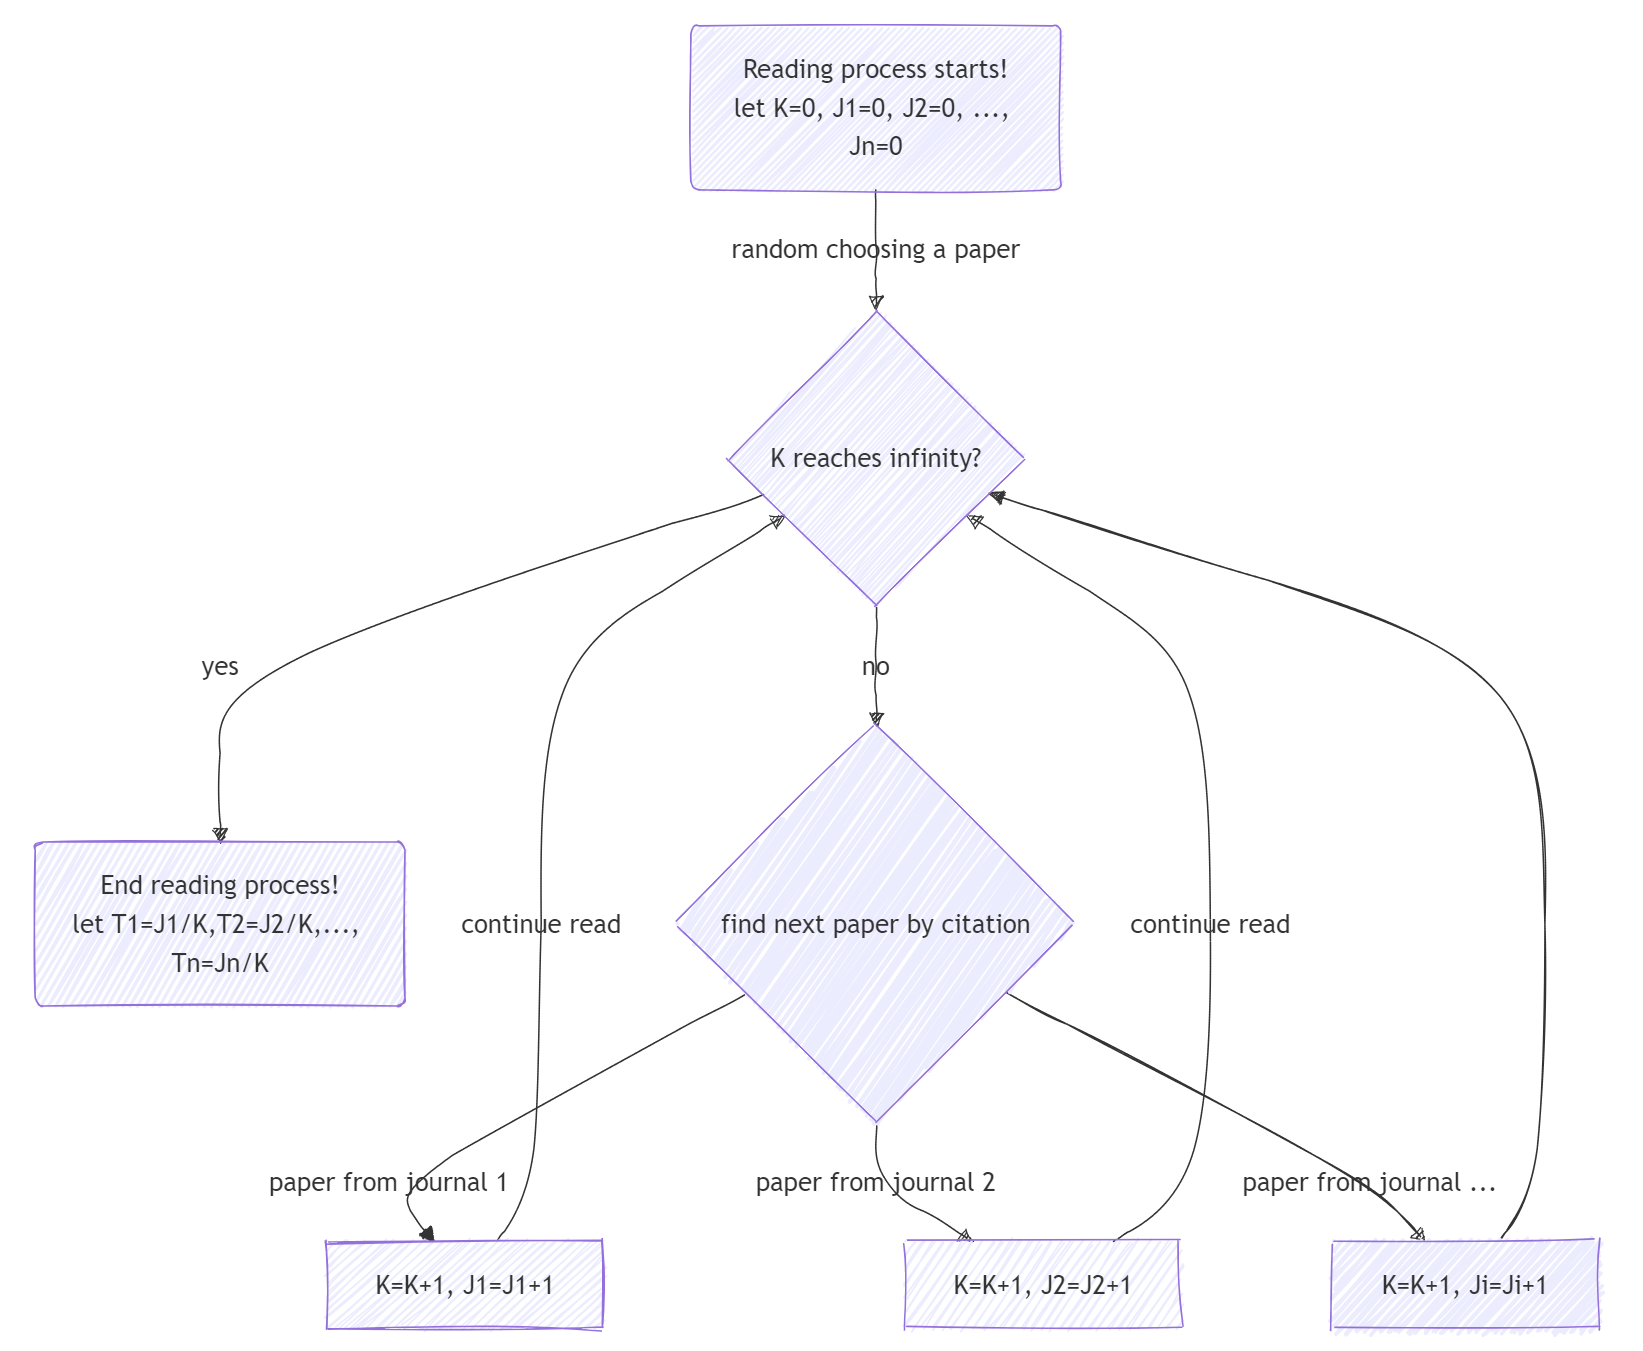
\includegraphics[width=\linewidth]{img/reader_time.png}  
    \caption{阅读者时间问题的过程}
    \label{fig:rt}
\end{figure}

插入超链接方法:\href{https://blog.liuyc.us.kg/}{例如我的主页} 

引用文献使用cite命令,需提前将bibtex格式加入ref.bib文件中,例如:llama3\cite{llama3},pangerank\cite{page1999pagerank}。

插入表格方法,表~\ref{tab:benchmark_claude3_test_gpt}给出了一个示例,可根据\href{https://www.tablesgenerator.com/}{https://www.tablesgenerator.com/}自行制作后粘贴到文档中。
\begin{table}[hbt]
\centering
\resizebox{\textwidth}{!} & 71\% & 64\% & 75.7\%  & 45.1\%  \\ \hline
\textbf{AMC 12}            & 5-shot CoT & \textbf{63} / 150 & 27 / 150 & 48 / 150 & 60 / 150 & 30 / 150  \\
\textbf{AMC 10}            & 5-shot CoT & \textbf{72} / 150 & 24 / 150 & 54 / 150 & 36 / 150 & 36 / 150  \\
\textbf{AMC 8}             & 5-shot CoT & 84 / 150 & 54 / 150 & 36 / 150 & - & -  \\ \hline
\textbf{GRE}(Quantitative) & 5-shot CoT & 159 & - & - & \textbf{163} & 147  \\
\textbf{GRE}(Verbal)       & 5-shot CoT & 166 & - & - & \textbf{169} & 154  \\
\textbf{GRE}(Writing)      & k-shot CoT & \textbf{5.0} (2-shot) & - & - & 4.0 (1-shot) & 4.0 (1-shot)  \\ \hline             
\end{tabular}%
}
\caption{Claude 3 评估结果对比}
\label{tab:benchmark_claude3_test_gpt}
\end{table}